As per the example from the lecture slides, pictured below, any arrows into a "plate" are repeated for all $N$ elements on the plate. Because all the arrows meet tail-to-tail at the $\pi$, $\mu$ and $\Sigma$ nodes, all paths are blocked between $z_1,...,z_n$. According to the rules of D-separation, they must then all be independent. Because $p(Z|X,\mu,\Sigma,\pi)$ is the combined probability of all $\in Z$, the general independence rule that $p(a,b) = p(a)p(b)$ must also apply, and thus we have shown that: $$p(Z|X,\mu,\Sigma,\pi) = \prod_{n=1}^N p(z_n|x_n, \mu, \Sigma, \pi)$$
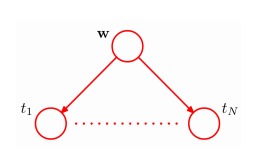
\includegraphics[width=0.5\linewidth]{plate.png}
